\documentclass[
  letterpaper,
  twocolumn,
  9pt,
  journal,
  final]{IEEEtran}

\usepackage[spanish,es-tabla]{babel}
\usepackage[utf8]{inputenc}
\usepackage{amsfonts}
\usepackage{amsmath}
\usepackage{amssymb}
\usepackage{amsxtra}
\usepackage{mathrsfs}
\usepackage{array}
\usepackage{tikz}
\usepackage{cite}
\usepackage{varioref}
\usepackage{float}
\usepackage{color}
\usepackage{colortbl}
\usepackage{enumerate}
\usepackage{rotating}
\usepackage{subcaption}
\usepackage{hyperref}
\usepackage{listings}
\usepackage{lipsum}
%\usepackage{flushend}
\usepackage{graphicx}
\usepackage{xcolor}
\hypersetup{
    colorlinks,
    linkcolor={red!50!black},
    citecolor={blue!50!black},
    urlcolor={blue!80!black}
}

\usepackage{lipsum}

\title{Tarea 4 - Procesamiento Digital de Imágenes}
\author{\textbf{Autor:} Pablo Yáñez Santibáñez - pablo.yanez@uai.cl}
%\author{\IEEEauthorblockN{Pablo Yáñez S.} - pablo.yanez@uai.cl}

% Levels to show in table of contents:
% \setcounter{tocdepth}{-1} % only parts
% \setcounter{tocdepth}{0}  % only parts and chapters
% \setcounter{tocdepth}{1}  % part,chapters,sections
\setcounter{tocdepth}{2}  % part,chapters,sections, subsections
% \setcounter{tocdepth}{3}  % part,chapters,sections, subsections,subsubsections
% \setcounter{tocdepth}{4}  % part,chapters,sections, subsections,subsubsections and paragraphs
% \setcounter{tocdepth}{5}  % part,chapters,sections, subsections, subsubsections, paragraphs and subparagraphs.

\begin{document}
\bstctlcite{IEEEexample:BSTcontrol}
\maketitle

% \begin{abstract}
% We propose \lipsum[1]
% \end{abstract}

\tableofcontents

% \listoffigures

% \listoftables

%%%%%%%%%%%%%%%%%%%%%%%%%%%%%%%%%%%%%%%%%%%%%%%%%%%%%%%%%%%%%%%%%%%%%%%%%%%%%%%%

\section{Introducción}

Para el desarrollo de este trabajo se descarga una imagen de Los Dientes de Navarino (Puerto Williams) del sitio \href{https://www.flickr.com/photos/whitewizard/7062826349/in/album-72157629780861323/}{Flickr}. Esta imagen es usada para las distintas actividades que se describen en este documento.

\begin{figure}[h!]
	\centering
	% 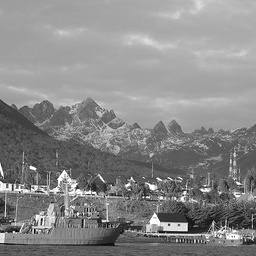
\includegraphics[width=0.6\linewidth, trim={0cm 0cm 0cm 5cm}, clip]{outs/gaussiano/img.jpg}
	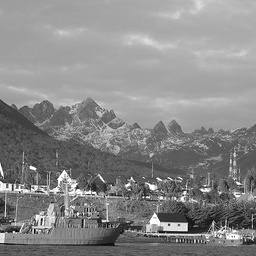
\includegraphics[width=0.4\linewidth, trim={0cm 0cm 0cm 0cm}, clip]{outs/gaussiano/img.jpg}
	\caption{Dientes de Navarino.}
	\label{dientes}
\end{figure}

\section{Marco Teórico} \label{teo}

\subsection{Imagen}

Se puede describir una imagen $g(x,y)$ como una composición de una imagen ideal $f(x,y)$ degradada por un proceso $h(x,y)$ más una componente de ruido $\eta(x,y)$.

\begin{align}
  g(x,y) = h(x, y) * f(x,y) + \eta(x,y)
\end{align}

Luego se tiene como objetivo poder recuperar la información de la imagen original a través de un proceso de restauración. La Figura \ref{restauracion} presenta un diagrama del proceso general.

\begin{figure}[h!]
	\centering
	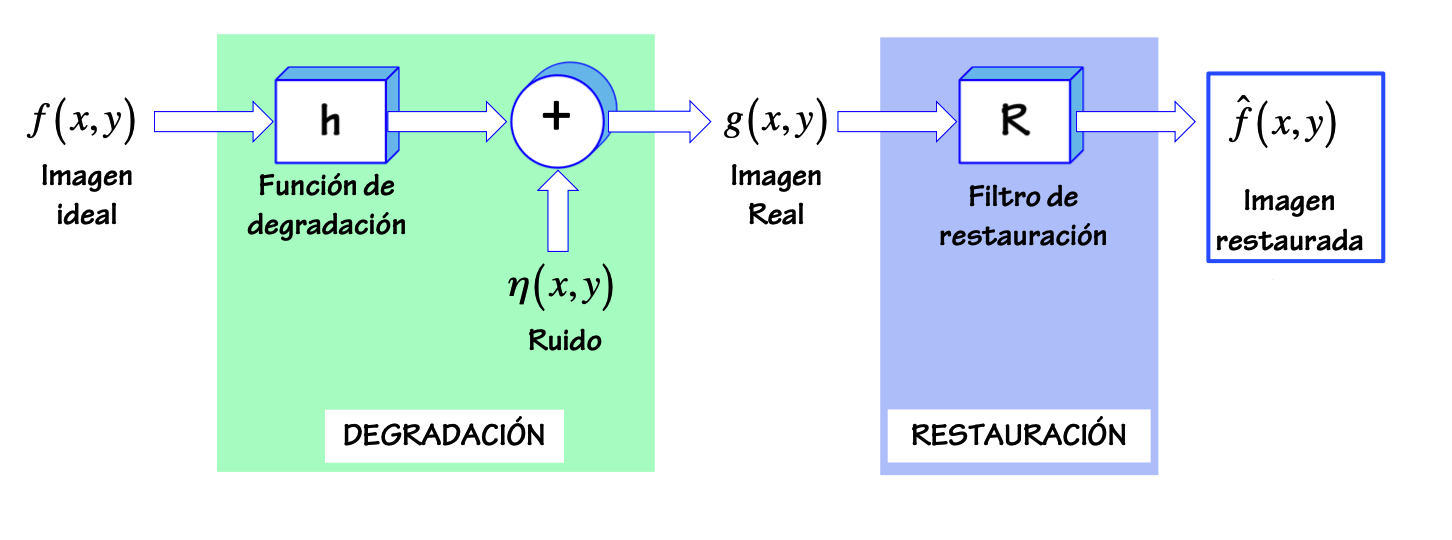
\includegraphics[width=0.8\linewidth, trim={0cm 0cm 1cm 0cmm}, clip]{other/restauracion.png}
	\caption{Diagrama proceso restauración \cite{carrasco3}.}
	\label{restauracion}
\end{figure}


\subsection{Ruido}

En las señales el ruido corresponde a una señal no deseada que se mezcla con la señal util. En el caso de las imágenes el ruido hace que un pixel de una imagen tome un valor que no corresponde al original. El ruido se puede catalogar de acuerdo a su naturaleza.

\subsubsection{Ruido Gaussiano:}
El ruido gaussiano se describe como una variable que sigue una distribución normal. En el caso de las imágenes, el ruido gaussiano se modela como un ruido aditivo, lo que significa que cada pixel es la suma de la información original más un una componente de ruido con distribución normal. La Figura \ref{gauss} muestra el efecto de aplicar ruido gaussiano a la imagen original con distintos valores de $\sigma$.

\begin{figure}[!tbh]
  \centering
  \begin{subfigure}[b]{.32\linewidth}
    \includegraphics[width=\linewidth]{outs/gaussiano/noisy_005.jpg}
    \caption{$\sigma=0.05$}\label{gauss_1}
  \end{subfigure}
  \begin{subfigure}[b]{.32\linewidth}
    \includegraphics[width=\linewidth]{outs/gaussiano/noisy_010.jpg}
    \caption{$\sigma=0.1$}\label{gauss_2}
  \end{subfigure}
  \begin{subfigure}[b]{.32\linewidth}
    \includegraphics[width=\linewidth]{outs/gaussiano/noisy_050.jpg}
    \caption{$\sigma=0.5$}\label{gauss_3}
  \end{subfigure}
  \caption{Imagen con ruido gaussiano.}
  \label{gauss}
\end{figure}

\subsubsection{Ruido Impulsional:}
El ruido impulsional corresponde a impulsos que contaminan la señal util con valores altos o bajos. En las imágenes el ruido impulsional hace que un pixel tome valores 0 o 255. Generalmente el ruido sigue una distribución normal. En el caso de que el ruido solo contamine con valores 0 se conoce como ruido pimienta, mientras que si contamina con valores 255 toma el nombre de ruido sal. La Figura \ref{impulsional} muestra ejemplos de ruido impulsional aplicado a la imagen original.

\begin{figure}[!tbh]
  \centering
  \begin{subfigure}[b]{.32\linewidth}
    \includegraphics[width=\linewidth]{outs/pimienta/noisy.jpg}
    \caption{Pimienta}\label{pimienta}
  \end{subfigure}
  \begin{subfigure}[b]{.32\linewidth}
    \includegraphics[width=\linewidth]{outs/sal/noisy.jpg}
    \caption{Sal}\label{sal}
  \end{subfigure}
  \begin{subfigure}[b]{.32\linewidth}
    \includegraphics[width=\linewidth]{outs/sal/noisy_sp.jpg}
    \caption{Sal y pimienta}\label{sal_pimienta}
  \end{subfigure}
  \caption{Imagen con ruido impulsional.}
  \label{impulsional}
\end{figure}

\subsubsection{Ruido Uniforme:}

El ruido uniforme hace que una señal pueda tomar un valor en un intervalo con una probabilidad constante. En el caso de una imagen, el ruido uniforme hace que la probabilidad de tomar cualquier valor de gris en un intervalo es constante. Ejemplos de aplicar ruido uniforme a la imagen original se presentan en la Figura \ref{uniforme}.

\begin{figure}[!tbh]
  \centering
  \begin{subfigure}[b]{.32\linewidth}
    \includegraphics[width=\linewidth]{outs/uniforme/noisy_b040.jpg}
    \caption{$a=10, b=40$}\label{uni1}
  \end{subfigure}
  \begin{subfigure}[b]{.32\linewidth}
    \includegraphics[width=\linewidth]{outs/uniforme/noisy_b060.jpg}
    \caption{$a=10, b=60$}\label{uni2}
  \end{subfigure}
  \begin{subfigure}[b]{.32\linewidth}
    \includegraphics[width=\linewidth]{outs/uniforme/noisy_b150.jpg}
    \caption{$a=10, b=150$}\label{uni3}
  \end{subfigure}
  \caption{Imagen con ruido uniforme.}
  \label{uniforme}
\end{figure}

\subsection{Modelos de Degradación}

\subsubsection{Turbulencia}

El modelo de turbulencia esta dado por (\ref{turb}). A través de la Transformada de Fourier el fénomeno de turbulencia puede modelarse como una multiplicación en el dominio de la frecuencia, donde el modelo de degradación esta dado por (\ref{turb_fourier}). La Figura \ref{turb} presenta tres ejemplos de aplicar la función de degradación a la imagen de la Figura \ref{dientes}.

\begin{align}
  g(x, y) &= h(x,y) * f(x,y) \label{turb} \\
  H(u,v) &= e ^ {-k (u^2 + v^2) \frac{5}{6}} \label{turb_fourier}
\end{align}

\begin{figure}[!tbh]
  \centering
  \begin{subfigure}[b]{.32\linewidth}
    \includegraphics[width=\linewidth]{outs/degradacion/turb_01.jpg}
    \caption{$k=0.001$}\label{turb1}
  \end{subfigure}
  \begin{subfigure}[b]{.32\linewidth}
    \includegraphics[width=\linewidth]{outs/degradacion/turb_05.jpg}
    \caption{$k=0.005$}\label{turb5}
  \end{subfigure}
  \begin{subfigure}[b]{.32\linewidth}
    \includegraphics[width=\linewidth]{outs/degradacion/turb_05.jpg}
    \caption{$k=0.009$}\label{turb9}
  \end{subfigure}
  \caption{Ejemplo de Turbulencia.}
  \label{turb}
\end{figure}

\subsubsection{Movimiento Lineal} \label{mov_lineal_sec}

El modelo de movimiento lineal replica el efecto de movimiento que ocurre cuando el objeto enfocado o el fotógrafo se mueve. El modelo de degradación en el dominio de la frecuencia se describe se según (\ref{mov_lineal}), donde los parámetros $a$, $b$ y $T$ son escalares. La Figura \ref{Movimiento_Lineal} presenta unos ejemplos de aplicar la degradación de movimiento lineal variando los parámetros de la función de degradación.

\begin{align}
  H(u,v) = T e^{-i\pi (ua + vb)} sinc( \pi (ua + vb)) \label{mov_lineal}
\end{align}

\begin{figure}[!tbh]
  \centering
  \begin{subfigure}[b]{.32\linewidth}
    \includegraphics[width=\linewidth]{outs/degradacion/mov_3_0_1.jpg}
    \caption{$a=3, b=0, T=1$}\label{mov1}
  \end{subfigure}
  \begin{subfigure}[b]{.32\linewidth}
    \includegraphics[width=\linewidth]{outs/degradacion/mov_0_3_1.jpg}
    \caption{$a=0, b=3, T=1$}\label{mov2}
  \end{subfigure}
  \begin{subfigure}[b]{.32\linewidth}
    \includegraphics[width=\linewidth]{outs/degradacion/mov_3_3_1.jpg}
    \caption{$a=3, b=3, T=1$}\label{mov3}
  \end{subfigure}
  \caption{Ejemplo de Movimiento Lineal.}
  \label{Movimiento_Lineal}
\end{figure}

\subsection{Filtros en el dominio espacial}

A continuación se describen los filtros en el dominio del espacio utilizados en este trabajo.

\subsubsection{Filtro Gaussiano}
Corresponde un filtro de la familia de filtros lineales. El filtro utiliza una máscara con distribución gaussiana normalizada.

\subsubsection{Filtro Max-Min}
Este filtro de la familia de filtros estadísticos. El filtro reemplaza el valor central de la máscara por el valor mínimo o máximo de las misma máscara.

\subsubsection{Filtro Ruido Local}
El filtro de ruido local pertenece a la familia de filtros adaptivos. El filtro modifica su comportamiento en función de las características locales de la máscara y del ruido global de la imagen. Este filtro es util cuando el ruido no es elevado y permite reducir el ruido gaussiano y uniforme si se ajustan bien sus parámetros.

\subsection{Filtro de Wiener}
El filtro de Wiener busca eliminar el ruido de una imagen, utilizando una aproximación del modelo de ruido y un parámetro de ajuste $k$. Una de las ventajas que tiene este filtro es que se puede utilizar un filtro conocido para filtar ruido producido por una función de degradación desconocida. La expresión en el dominio de la frecuencia de este filtro se presenta en (\ref{wiener}).

\begin{align}
  \hat{F}(u,v) = \left( \frac{| H(u,v)|^2 }{ H(u,v) (|H(u,v)|^2 +k)  }    \right ) G(u,v) \label{wiener}
\end{align}

\subsection{Filtro Paramétrico}
El filtro paramétrico posee una formulación similar a la del Filtro de Wiener, pero en vez de utilizar un factor de ajuste utiliza una matriz de filtraje. Su formulación se presenta en \ref{parametrico}.

\begin{align}
  \hat{F}(u,v) = \left( \frac{H(u,v)|^* }{ |H(u,v)|^2 + \gamma |P(u,v)|^2)} \right ) G(u,v) \label{parametrico}
\end{align}

\section{Desarrollo}

A continuación se presenta distintas técnicas de filtrado para las imágenes mostradas en la sección \ref{teo}.

\subsection{Ruido Gaussiano}

Para filtrar las imágenes de la Figura \ref{gauss} se utiliza un filtro gaussiano, probando distintos valores para el tamaño de la mascara a utilizar. En la Figura \ref{gauss_filtrado} se presentan los resultados de aplicar el filtro a tres imágenes. La correspondencia entre las imágenes de presenta en la Tabla \ref{tab_gauss}.

\begin{table}[!tbh]
  \centering
  \caption{Filtrado Ruido Gaussiano} \label{tab_gauss}
  \begin{tabular}{cccl}
  Imagen & Ventana & Var. Estimada & Imagen Filtrada \\ \hline
  Figura \ref{gauss_1}     & $3\times3$        & 2.2            & Figura \ref{gauss_filtrado_1}               \\
  Figura \ref{gauss_2}     & $5\times5$      & 2.2            & Figura \ref{gauss_filtrado_2}               \\
  Figura \ref{gauss_3}     & $7\times7$      & 2.2            & Figura \ref{gauss_filtrado_3}
  \end{tabular}
\end{table}

\begin{figure}[!tbh]
  \centering
  \begin{subfigure}[b]{.32\linewidth}
    \includegraphics[width=\linewidth]{outs/gaussiano/filtered_5_3x3.jpg}
    \caption{Máscara $3\times3$}\label{gauss_filtrado_1}
  \end{subfigure}
  \begin{subfigure}[b]{.32\linewidth}
    \includegraphics[width=\linewidth]{outs/gaussiano/filtered_10_5x5.jpg}
    \caption{Máscara $5\times5$}\label{gauss_filtrado_2}
  \end{subfigure}
  \begin{subfigure}[b]{.32\linewidth}
    \includegraphics[width=\linewidth]{outs/gaussiano/filtered_50_7x7.jpg}
    \caption{Máscara $7\times7$}\label{gauss_filtrado_3}
  \end{subfigure}
  \caption{Filtrado imágenes de Figura \ref{gauss}.}
  \label{gauss_filtrado}
\end{figure}

Se puede apreciar que el filtro efectivamente logra reducir el ruido para el caso de las imágenes generadas con ruido gaussiano con valores de $\sigma=0.05$ y $\sigma=0.1$. En el caso de la imagen con una mayor presencia de ruido, no es posible recuperar la imagen original.

\subsection{Ruido Impulsional}

Se aplica un filtro máximo y mínimo para filtrar las Figuras \ref{pimienta} y \ref{sal} respectivamente. En ambos caso se logra eliminar la componente no deseada de la imagen, con una pequeña perdida en la definición de los detalles. Resulta de interés destacar que el filtro máximo tiende a aclara la imagen, mientras que el filtro mínimo la oscurece.

\begin{figure}[!tbh]
  \centering
  \begin{subfigure}[b]{.4\linewidth}
    \includegraphics[width=\linewidth]{outs/pimienta/filtered_3x3.jpg}
    \caption{Pimienta - Máscara $3\times3$}\label{pimienta_filtrado}
  \end{subfigure}
  \begin{subfigure}[b]{.40\linewidth}
    \includegraphics[width=\linewidth]{outs/sal/filtered_2x2.jpg}
    \caption{Sal - Máscara $3\times3$}\label{sal_filtrado}
  \end{subfigure}
  \caption{Filtrado imágenes de la Figura \ref{impulsional}.}
  \label{gauss_filtrado}
\end{figure}

\subsection{Ruido Uniforme}

Para el filtrado del ruido uniforme se utiliza un filtro de ruido local. Se prueba distintos valores para la varianza estimada del filtro, fijando el tamaño de la mascara ($5 \times 5$).

\begin{table}[!tbh]
  \centering
  \caption{Filtrado Ruido Uniforme} \label{tab_gauss}
  \begin{tabular}{cccl}
  Imagen & Ventana & Var. Estimada & Imagen Filtrada \\ \hline
  Figura \ref{uni1}     & $5\times5$      & 0.001            & Figura \ref{uni_filtrado_1}               \\
  Figura \ref{uni2}     & $5\times5$      & 0.003            & Figura \ref{uni_filtrado_2}               \\
  Figura \ref{uni3}     & $5\times5$      & 0.005            & Figura \ref{uni_filtrado_3}
  \end{tabular}
\end{table}

\begin{figure}[!tbh]
  \centering
  \begin{subfigure}[b]{.32\linewidth}
    \includegraphics[width=\linewidth]{outs/uniforme/filtered_040_0.001.jpg}
    \caption{Var. est.: $0.001$}
    \label{uni_filtrado_1}
  \end{subfigure}
  \begin{subfigure}[b]{.32\linewidth}
    \includegraphics[width=\linewidth]{outs/uniforme/filtered_060_0.003.jpg}
    \caption{Var. est.: $0.003$}
    \label{uni_filtrado_2}
  \end{subfigure}
  \begin{subfigure}[b]{.32\linewidth}
    \includegraphics[width=\linewidth]{outs/uniforme/filtered_150_0.005.jpg}
    \caption{Var. est.: $0.005$}
    \label{uni_filtrado_3}
  \end{subfigure}
  \caption{Filtrado imágenes de la Figura \ref{uniforme}.}
  \label{uniforme_filtrado}
\end{figure}

Se observa que en el caso de las dos primeras imágenes se logra reducir el ruido uniforme introducido. En el caso de la tercera imagen, el objetivo no se logra, ya que la cantidad de ruido es muy elevada.

\subsection{Degradación}

Para el desarrollo de esta sección se utiliza la imagen dada según el enunciado de la tarea. La imagen a restaurar se presenta en la Figura \ref{cameraman_deg}.

\begin{figure}[!tbh]
  \centering
  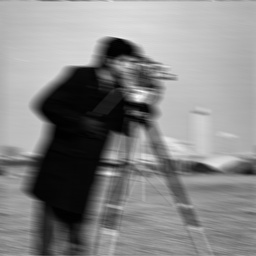
\includegraphics[width=0.4\linewidth]{inputs/cameraman_noisy.jpg}
  \caption{Imagen degradada mediante función desconocida.}
  \label{cameraman_deg}
\end{figure}


\subsubsection{Filtro de Wiener}

Se asume un modelo de degradación de movimiento lineal como el indicado en \ref{mov_lineal_sec}. Se usa como $H(u,v)$ un filtro pasabajos de Butterworth de orden 2 con frecuencia de corte $f=30$.

\begin{figure}[!tbh]
  \centering
  \includegraphics[width=0.4\linewidth]{outs/wiener/filtered__23.jpg}
  \caption{Imagen filtrada usando filtro de Wiener. $k=0.079$.}
  \label{wiener_fitlro}
\end{figure}

El resultado no logra remover completamente el ruido de la imagen, lo que se puede atribuir a una mala elección de los parámetros de filtro, así como del valor de $k$.

\subsubsection{Filtro de Paramétrico}

Al igual que el caso del filtro de Wiener se utiliza un filtro de Butterworth de orden 1 y frecuencia de corte $f=15$. El resultado de filtrar la imagen se presenta en la Figura \ref{param_filtrado}.

\begin{figure}[!tbh]
  \centering
  \includegraphics[width=0.4\linewidth]{outs/param/filtered__22.jpg}
  \caption{Imagen filtrada usando filtro paramétrico. $gamma=0.075$.}
  \label{param_filtrado}
\end{figure}

Nuevamente no se logra una satisfactoria restauración de la imagen, por lo que hay que evaluar los parámetros usados para así conseguir una mejor imagen.

\section{Código}

Se adjunta dos códigos para reproducir los resultados presentados en este documento. Para su ejecucion basta con ejecutar cada uno de los scripts utilizando el interprete de python.

\begin{verbatim}
python pablo_yanez_t4_parte1_gaussiano.py
python pablo_yanez_t4_parte1_pimienta.py
python pablo_yanez_t4_parte1_sal.py
python pablo_yanez_t4_parte1_uniforme.py
python pablo_yanez_t4_parte2_parametrico.py
python pablo_yanez_t4_parte2_wiener.py
\end{verbatim}


%%%%%%%%%%%%%%%%%%%%%%%%%%%%%%%%%%%%%%%%%%%%%%%%%%%%%%%%%%%%%%%%%%%%%%%%%%%%%%%%
% Bibliography
\nocite{*}
\bibliographystyle{IEEEtran}
\bibliography{bibliography}


\end{document}
